%%%%%%%%%%%%%%%%%%%%%%%%%%%%%%%%%%%%%%%%%
% Beamer Presentation
% LaTeX Template
% Version 1.0 (10/11/12)
%
% This template has been downloaded from:
% http://www.LaTeXTemplates.com
%
% License:
% CC BY-NC-SA 3.0 (http://creativecommons.org/licenses/by-nc-sa/3.0/)
%
%%%%%%%%%%%%%%%%%%%%%%%%%%%%%%%%%%%%%%%%%

%----------------------------------------------------------------------------------------
%	PACKAGES AND THEMES
%----------------------------------------------------------------------------------------

\documentclass{beamer}
%\usepackage{cite}

\mode<presentation> {

% The Beamer class comes with a number of default slide themes
% which change the colors and layouts of slides. Below this is a list
% of all the themes, uncomment each in turn to see what they look like.

%\usetheme{default}
%\usetheme{AnnArbor}
%\usetheme{Antibes}
%\usetheme{Bergen}
%\usetheme{Berkeley}
%\usetheme{Berlin}
%\usetheme{Boadilla}
%\usetheme{CambridgeUS}
%\usetheme{Copenhagen}
\usetheme{Darmstadt}
%\usetheme{Dresden}
%\usetheme{Frankfurt}
%\usetheme{Goettingen}
%\usetheme{Hannover}
%\usetheme{Ilmenau}
%\usetheme{JuanLesPins}
%\usetheme{Luebeck}
%\usetheme{Madrid}
%\usetheme{Malmoe}
%\usetheme{Marburg}
%\usetheme{Montpellier}
%\usetheme{PaloAlto}
%\usetheme{Pittsburgh}
%\usetheme{Rochester}
%\usetheme{Singapore}
%\usetheme{Szeged}
%\usetheme{Warsaw}

% As well as themes, the Beamer class has a number of color themes
% for any slide theme. Uncomment each of these in turn to see how it
% changes the colors of your current slide theme.

%\usecolortheme{albatross}
%\usecolortheme{beaver}
%\usecolortheme{beetle}
%\usecolortheme{crane}
%\usecolortheme{dolphin}
%\usecolortheme{dove}
%\usecolortheme{fly}
%\usecolortheme{lily}
%\usecolortheme{orchid}
%\usecolortheme{rose}
%\usecolortheme{seagull}
\usecolortheme{seahorse}
%\usecolortheme{whale}
%\usecolortheme{wolverine}

%\setbeamertemplate{footline} % To remove the footer line in all slides uncomment this line
%\setbeamertemplate{footline}[page number] % To replace the footer line in all slides with a simple slide count uncomment this line

%\setbeamertemplate{navigation symbols}{} % To remove the navigation symbols from the bottom of all slides uncomment this line
}
\usepackage{tabstackengine}
\usepackage{media9}
\usepackage{graphicx} % Allows including images
\usepackage{booktabs} % Allows the use of \toprule, \midrule and \bottomrule in tables
\usepackage{parskip}
\usepackage{caption}
\usepackage{subcaption}
\usepackage{tikz}
\renewcommand{\arraystretch}{1.5}
%\usepackage{cite}



%----------------------------------------------------------------------------------------
%	TITLE PAGE
%----------------------------------------------------------------------------------------

\title[Laplacian Matrix]{LAPLACIAN MATRIX OF A NETWORK AND APPLICATIONS} % The short title appears at the bottom of every slide, the full title is only on the title page


\author[Alice Nanyanzi] {\includegraphics[width=0.4\textwidth]{images/AIMSlogo.png}\hspace*{3.75cm}~%
	\includegraphics[width=0.3\textwidth]{images/su1.png} \\
	\vspace{0.75cm}
	Alice Nanyanzi \\
	\textit{alicenanyanzi@aims.ac.za}\\
	\vspace{0.4cm}
	\textbf{Supervisors:}\\
	 Prof. Franck Kalala Mutombo$^1$ \& Dr. Simukai Utete$^2$\\ 
	 \vspace{0.4cm}
	 $1.$ AIMS,Senegal \& University of Lubumbashi\\
	 $2.$ AIMS,South Africa \& Stellenbosch University
} % Your name
\institute[AIMS-SU] % Your institution as it will appear on the bottom of every slide, may be shorthand to save space
{
%African Insitute for Mathematical Sciences (AIMS)-Stellenbosch University \\ % Your institution for the title page
% logo of my universit
%\vspace{0.5 cm}
% Your email address
}
\date{\today} % Date, can be changed to a custom date


\begin{document}

\begin{frame}[noframenumbering, plain]
\titlepage % Print the title page as the first slide
\end{frame}

\begin{frame}
\frametitle{} % Table of contents slide, comment this block out to remove it
\tableofcontents % Throughout your presentation, if you choose to use \section{} and \subsection{} commands, these will automatically be printed on this slide as an overview of your presentation
\end{frame}

%----------------------------------------------------------------------------------------
%	PRESENTATION SLIDES
%----------------------------------------------------------------------------------------

%------------------------------------------------

\section{Over view of Networks} % Sections can be created in order to organize your presentation into discrete blocks, all sections and subsections are automatically printed in the table of contents as an overview of the talk
%------------------------------------------------

%\subsection{Subsection Example} % A subsection can be created just before a set of slides with a common theme to further break down your presentation into chunks

%Today, many systems in real world are composed of components which are linked to each other to form complex systems. These systems include technological systems, ecological systems, social systems, biological systems among others. 
%Recently, researchers have been involved in the study of various complex systems so as to address real world problems such as financial market crushes, traffic congestion, epidermic breakouts, computer virus spread, terrorist attacks, etc.
%It is therefore of utmost importance to study the behaviour and properties of these systems. This is achieved by representing complex systems by complex networks whose structural properties are then studied.
%in order to find solutions to issues such as financial market crushes, traffic congestion, epidermic breakouts, computer virus spread, terrorist attacks, etc. 
% Network theory is one of the approaches used in studying complex systems by representing a complex system as a complex network followed by understanding the structural properties of the complex network. 
 %The Laplacian matrix is one of the many matrices used to represent networks and it provides useful information on the properties of complex networks.
%Some of the applications  include diffusion process on networks, centrality measures(Laplacian centrality), consensus in networks etc. We f
%The Laplacian matrix has various applications in the study of networks. We consider two of the applications that is application to centrality measure and diffusion on networks.
\begin{frame}
	\frametitle{Introduction to Networks}
	
	\begin{itemize}
		\item \textcolor{blue}{Intuition of Networks}
		
		Whenever one mentions the word 'network', one normally thinks of an interconnection of items or things.
		\pause
		\item Did you know?
			\begin{figure}[!h]
				\centering
				\includegraphics[width=0.75\textwidth]{images/networkeverywhere.png}
			\end{figure}
		\end{itemize}
	\end{frame}

   \begin{frame}
   	\frametitle{Complexity \& Complex Systems}
   
   	 \begin{columns}
   		\begin{column}{0.5\textwidth}
   			
   			"I think the next century will be a century of complexity" - Stephen Hawking
   			
   		\end{column}
   		\begin{column}{0.5\textwidth} 
   			\begin{center}
   				\includegraphics[width=0.65\textwidth]{images/stephen-hawking.jpg}
   			\end{center}
   		\end{column}
   	\end{columns}
     \end{frame}
%   \item Complexity, a scientific theory which asserts that  systems display behaviour phenomena that are completely inexplicable by an conventional analysis of a system's constituent components. These phenomena commonly referred to as emergent behaviour, seem to occur in many complex systems involving living organisms, such as a stock market or human brain.
%   \item 
%   \end{itemize}
 


\begin{frame}{Complexity and Complex Systems cont...}
\begin{columns}
	\begin{column}{0.65\textwidth}
		\begin{center}
			\includegraphics[width=1.0\textwidth]{images/complexity.png}
		\end{center}
		
	\end{column}
	\begin{column}{0.45\textwidth} 
		\begin{center}
			\includegraphics[width=0.65\textwidth]{images/systemcomponents.png}
		\end{center}
	\end{column}
\end{columns}
\end{frame}

\begin{frame}{Complex Networks}
	\begin{itemize}
		\item Complex Networks represent skeletons of complex systems
		\item Complex networks exhibit a \textcolor{red}{non-trivial topology}
	\end{itemize}
	\begin{figure}[!h]
		\centering
		\includegraphics[width=0.75\textwidth]{images/complex-nets.png}
	\end{figure}
\end{frame}




\begin{frame}{Network Approach to Complex System Study}
	
	\begin{figure}[!h]
		\centering
		\includegraphics[width=0.60\textwidth]{images/abstract-diagram.pdf}
		\caption{Illustration of the process of network theory approach}
		%\label{stardifn-graph}
	\end{figure}
	
%	\begin{table}
%		\begin{tabular}{p{3.5cm} p{3cm} p{3.5cm}}	
%				\includegraphics[width=0.3\textwidth]{images/Konigsberg_bridges.png}
%			 & \includegraphics[width=0.3\textwidth]{images/mapping.png}  & \includegraphics[width=0.35\textwidth]{images/nodemapbridges.jpg} \\
%			  \includegraphics[width=0.12\textwidth]{images/arrow-up.jpg}& &
%			  \includegraphics[width=0.3\textwidth]{images/understanding.png}\\
%			  \includegraphics[width=0.35\textwidth]{images/properties.png}&  \includegraphics[width=0.12\textwidth]{images/arrow-back.jpg}&\includegraphics[width=0.3\textwidth]{images/matrix-rep.png} 
%		\end{tabular}
%	\end{table}
\end{frame}

%------------------------------------------------



\begin{frame}{Real-world Networks}
	\begin{figure}[!h]
		\centering
		\begin{subfigure}[b]{0.3\textwidth}
			\includegraphics[width=\textwidth]{images/Steve-Jurvetson.jpg}
			\caption{Internet}
			%\label{stardifn-graph}
		\end{subfigure}\qquad
		\begin{subfigure}[b]{0.3\textwidth}
			\includegraphics[width= \textwidth]{images/yeastprotein-protein-interactions.jpeg}
			\caption{Protein-Protein }
			%\label{stardifn-plot}
		\end{subfigure}\\
		\begin{subfigure}[b]{0.3\textwidth}
			\includegraphics[width=\textwidth]{images/food-web-2.png}
			\caption{Food web}
			%\label{regdifn-graph}
		\end{subfigure}~
		\begin{subfigure}[b]{0.3\textwidth}
			\includegraphics[width= \textwidth]{images/citation.jpg}
			\caption{Citation network}
			%\label{regdifn-plot}
		\end{subfigure}
	\end{figure}
Source: www.wikipedia.com
\end{frame}

\begin{frame}{AIMS,SA 2016-2017 Friendship Network}
	\begin{figure}[!h]
		\includegraphics[width= \textwidth]{images/AIMS,SouthAfricaNetwork.png}
		\caption{AIMS,SA 2016-2017 Friendship Network: December (left) and April (right). The size of each node is proportional to
			in-degree (close friends).}
	\end{figure}
Source: Emily Muller, Master's Thesis
\end{frame}

\section{Laplacian Matrix}
\begin{frame}{Laplacian Matrix}
	\begin{block}{Definition}
		For a simple undirected graph;
		
			\begin{equation}
			L= D-A,
			\end{equation} 
		where $D$ is the $diag(k_i)$ and $A_{i,j}=1$ if $i~j$ and $0$ otherwise.\\
		\vspace{0.5 cm}
		The entries of $L$ are given by\\
    	\begin{equation}
    	L_{i,j} = \begin{cases}
    	k_i & \text{ if }  i=j\\
    	-1  & \text{if } i \neq j \text{ and } i ~ j \\
    	0 & \text{otherwise},
    	\end{cases}
    	\end{equation}
    	where $k_i$ denotes the degree of node $i$ (Estrada, 2011).
    \end{block}
\end{frame}

\begin{frame}{Spectrum of the Laplacian Matrix}
	\only<1->{\begin{block}{Spectrum}
		Spectrum of a matrix is a set eigenvalues and their multiplicities. Let $\lambda_i$ denote the eigenvalues of the Laplacian matrix. Considering the nondecreasing order: $\lambda_n  \geq \lambda_{n-1} \geq  \cdots \geq \lambda_2 \geq \lambda_1 =0 $
		\end{block}}
	
	  \only<2> {\begin{block}{Insights from spectrum}
	    \begin{itemize}
	    	\item The multiplicity of $0$ as an eigenvalue of $\mathbf{L}$ is equal to the number of connected components in the network.
	    	\item  A network, G, is connected if its second smallest eigenvalue is nonzero. That is, $\lambda_2> 0$ if and only if $G$ is connected. The eigenvalue $\lambda_2$ is thus called the algebraic connectivity of a network, $a(G)$ (Estrada, 2011).
	    \end{itemize}
	\end{block}}

\end{frame}
\section{Applications of Laplacian Matrix}
\begin{frame} {Applications of Laplacian Matrix}
	\begin{itemize}
		\item \textcolor{blue}{Centrality measure}
		\item \textcolor{blue}{Diffusion on network}
		\item Consensus in multi-agent systems
		\item Synchronization, etc  
	\end{itemize}
\end{frame}
\begin{frame}{Centrality Measures}
	In networks, centrality is the measure how important/central a node is, in the network (Newman, 2010). There exists various measures such as:
	\begin{itemize}[<+(1)->]
		\item \textcolor{green}{Degree} centrality: Power through links
		\item \textcolor{green}{Closeness} centrality: Power through proximity to others
		\item \textcolor{green}{Betweenness} centrality: Ability to act as a bridge
		\item \textcolor{green}{Eigenvector} centrality: Improvement in degree centrality
		\item \textcolor{green}{Subgraph} centrality: Participation of a node in subgraphs in network
		\item \textcolor{red}{Laplacian} centrality : Impact of deactivation/removal of a node from the network.
	\end{itemize} 
\end{frame}
\subsection{Laplacian Centrality}
\begin{frame}{Laplacian Centrality: motivation}
	\begin{itemize}
%		\item Work presented is based on the paper: Laplacian centrality: A new centrality measure for weighted networks  by Qi et al., 2012.
%		\pause
		\item There is a growing need for centrality measures for weighted networks since these networks contain rich information (Qi et al., 2012).
		\vspace{0.2cm}
%		\pause
%		\item  Standard centrality measures (degree, closeness, betweenness) have been extended to cater for weighted networks, however, these measures either capture the local or global characterisation of networks (T.Opsahl '2009, Newman '2001, A.Barrat '2004, U.Brandes '2001). 
%		\vspace{0.2cm}
		\pause
		\item The Laplacian centrality is a measure between local and global (i.e intermediate) characterisation of the centrality of a node.
	    \end{itemize}
\end{frame}

\begin{frame}{Laplacian Centrality Cont....}
	\begin{block}{Laplacian Energy of a Network}
		The importance of a node is determined by the ability of the network to respond to the deactivation of a node from the network. \\
		\vspace{0.4cm}
		The response is quantified by the relative drop in Laplacian energy ($E_{L}$) of the network (Qi et al., 2012).
        \vspace{0.4cm}
		
		\begin{equation}
		E_L(G) = \sum_{i=1}^n \lambda_i ^2 = \sum_{i=1}^n x_i^2 + 2 \sum_{i<j} w_{i,j}^2,
		\end{equation}
		 where $x_i's$ are vertex sums and $w_{ij}$ are weights of edges between vertices $i$ and $j$ (Qi et al., 2012).
	\end{block}
\end{frame}

\begin{frame}{Mathematical Formulation of Laplacian Centrality}
Mathematically, Laplacian centrality for a node $i$ in network $G$ is given by (Qi et al., 2012) \\
\vspace{0.2cm}
\begin{equation}
C_L(v_i,G) = \frac{(\Delta E)_i}{E_L(G)} = \frac{E_L(G) - E_L(G_i)}{E_L(G)},
\label{lapcent}
\end{equation}
where \\
$E_L(G)$ - Laplacian energy of network $G$.\\
$E_L(G_i)$ - Laplacian energy of network $G$ on removal of node $i$
\end{frame}

\begin{frame}{Graph Theoretical Interpretation of Laplacian Centrality}
Expressing Equation \ref*{lapcent} in terms of $2$-walks of the node $i$ gives
\begin{equation}
(\Delta E)_i = 2\cdot NW_{2} ^M(v_i) + 2 \cdot NW_{2} ^E(v_i) + 4 \cdot NW_{2} ^C(v_i), 
\end{equation}
where 
\begin{itemize}
\item	$NW_{2} ^C(v_i)$ -  closed $2$-walks containing vertex $v_i$,
\item $NW_{2} ^E(v_i)$   -  non-closed $2$-walks with$v_i$ as one of the end points,
\item $NW_{2} ^M(v_i)$  - non-closed $2$-walks with $v_i$ as the middle point.
\end{itemize}


\begin{figure}[!h]
	\centering
	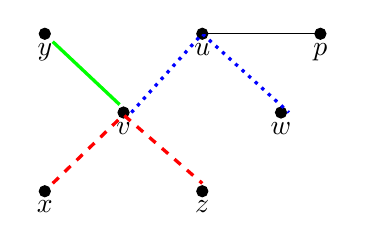
\begin{tikzpicture}
	\filldraw
	(0,0) circle (2pt) node[align=left, below] {$x$} 
	(1,1) circle (2pt) node[align=center, below] {$v$}    
	(0,2) circle (2pt) node[align=right,  below] {$y$}
	(2,2) circle (2pt) node[align=right,  below] {$u$}
	(2,0) circle (2pt) node[align=center, below] {$z$}  
	(3,1) circle (2pt) node[align=right,  below] {$w$}
	(3.5,2) circle (2pt) node[align=right,  below] {$p$};
	\draw[red, dashed, very thick] (0.1,0.1) -- (1.0,0.97) -- (2.0,0.1);	
	\draw[blue,dotted, very thick] (1.1,1.0) -- (2.0,2.0) -- (3.1,1.0);
	\draw[green,solid, very thick] (0.95,1.1) -- (0.1,1.9) -- (0.95,1.1);	
	\draw[] (2,2) -- (3.5,2);		
	\end{tikzpicture}
	\caption{$2$-walks at node $v$}
\end{figure}

\end{frame}

\begin{frame}{Application to Zachary's Karate Network}
		\begin{itemize}
		\item \textbf{The Zachary's Karate Network} was created from a dataset formed by observation of $34$ members of a karate club over two years. Misunderstandings within the group led to a split into two groups, one led by the Administrator ($1$) and the other by the instructor ($34$).
		\vspace{0.2cm}
		\pause
		\item \textcolor{green}{Nodes} represent \textcolor{green} {players} in both groups 
		\item \textcolor{green}{Edges} represent \textcolor{green}{interactions} outside karate activities.
		\vspace{0.2cm}
		\pause
		\item The \textcolor{green}{weights} on the edges correspond to various \textcolor{green}{activities} of interactions between players
		\vspace{0.2cm}
		\pause
		\item Database Source:
		 \url{http://nexus.igraph.org/api/dataset_info?id=1&format=html}
		
		\end{itemize}
		
\end{frame}

\begin{frame}{Zachary's Karate Network cont...}
%\textbf{The Zachary's Karate Network} was created from a dataset formed by observation of $34$ members of a karate club over two years. Misunderstandings within the group led to a split into two groups, one led by the Administrator ($1$) and the other by the instructor ($34$).
	\begin{figure}[!h]
		\centering
			\includegraphics[width=0.95\textwidth]{images/zachvisual.png}
			\caption{Zachary's Karate Network}
			%\label{stardifn-graph}
	\end{figure}
\end{frame}

%\begin{frame}{Centrality rankings of the Zachary's Karate network}	
%	\begin{table}[!h]
%		\centering
%		\Large
%		\setlength{\tabcolsep}{14pt}
%		\scalebox{0.45}{
%			\begin{tabular}{|l| r r c c| r r r r|}
%				\hline 
%				&  & Scores & & & & Ranks & & \\
%				\hline
%				Node & Degree & Betweenness & Closeness & Laplacian & Degree & Betweenness & Closeness & Laplacian \\ 
%				\hline 
%				$\mathbf{n_0}$ & \textbf{42} & \textbf{250.15} & \textbf{0.2538} & \textbf{0.2544} & \textbf{2} & \textbf{1} & \textbf{1} & \textbf{2} \\ 
%				$n_1$ & 29 & 33.80 & 0.2000 & 0.1725 & 5 & 8 & 8 & 5\\ 
%				$n_2$ & 33 & 36.65 & 0.1964 & 0.2166  & 4 & 6 & 11 & 4\\ 
%				$n_3$ & 18 & 1.33 & 0.1765& 0.0965  & 8 & 18 & 17 & 10 \\
%				$\vdots$ & $\vdots$ & $\vdots$ & $\vdots$ & $\vdots$  & $\vdots$ & $\vdots$ & $\vdots$ & $\vdots$\\
%%$n_4$ & 8 & 0.50 &0.1528 & 0.0350 & 18 & 21 & 28 & 22\\ 
%%$n_5$ & 14 &15.50 & 0.1521 & 0.0571 & 11 & 10 & 29 & 16\\ 
%%				$n_6$ & 13 & 15.50 & 0.1535 & 0.0541 & 13 & 10 & 27 & 18 \\ 
%%				$n_7$ & 13 &0.00 & 0.1823 & 0.0789 & 13 & 24 & 16 & 11 \\ 
%%				$n_8$ & 17 & 13.10 & 0.1988 & 0.1222 & 9 & 12 & 10 & 8\\ 
%%				$n_9$ & 3 & 7.28 & 0.1908 & 0.0218 & 31 & 14 & 13 & 30\\ 
%%				$n_{10}$ & 8 &0.50&  0.1755 & 0.0309  & 18 & 21 & 19 & 24\\ 
%%				$n_{11}$ & 3 & 0.00 & 0.1460 & 0.0216 & 31 & 24 & 30 & 31 \\ 
%%				$n_{12}$ & 4 & 0.00 & 0.2050 & 0.0174  & 28 & 24 & 5 & 33\\ 
%%				$n_{13}$ & 17 & 1.20 & 0.1908 & 0.1189 & 9 & 19 & 13 & 9\\ 
%%				$n_{14}$ & 5 & 0.00 &  0.1710 & 0.0366 & 25 & 24 & 22 & 20\\ 
%%				$n_{15}$ & 7 & 0.00 & 0.1375 & 0.0549  & 20 & 24 & 32 & 17\\ 
%%				$n_{16}$& 6 & 0.00 & 0.1086 & 0.0173   & 22 & 24 & 34 & 34\\ 
%%				$n_{17}$ & 3 & 16.10 &  0.1930 & 0.0192 & 31 & 9 & 12 & 32\\ 
%				$n_{18}$ & 3 & 3.00 &  0.1875 & 0.0226  & 31 & 16 & 15 & 29\\ 
%				$\mathbf{n_{19}}$ & \textbf{5} & \textbf{127.07} &  \textbf{0.2481} & \textbf{0.0331} & \textbf{25} & \textbf{3} & \textbf{3} & \textbf{23}\\ 
%				$n_{20}$ & 4 & 0.00 &  0.2037 & 0.0280  & 28 & 24 & 6 & 26\\ 
%				$n_{21}$ & 4 & 0.00 &  0.1765 & 0.0246  & 28 & 24 & 17 & 27\\ 
%				$n_{22}$ & 5 & 0.00 & 0.1587 & 0.0382  & 25 & 24 & 24 & 19\\ 
%				%$n_{23}$ & 21 & 1.00 & 0.1387 & 0.1294  & 6 & 20 & 31 & 7\\ 
%				$\vdots$ & $\vdots$ & $\vdots$ & $\vdots$ & $\vdots$  & $\vdots$ & $\vdots$ & $\vdots$ & $\vdots$\\ 
%%				$n_{24}$& 7 & 33.83 &  0.1579 & 0.0227  & 20 & 7 & 25 & 28\\ 
%%				$n_{25}$& 14 & 0.50 &  0.1236 & 0.0645  & 11 & 21 & 33 & 15 \\ 
%%				$n_{26}$ & 6 & 0.00 &  0.1692 & 0.0282  & 22 & 24 & 23 & 25\\ 
%%				$n_{27}$& 13 & 6.50 & 0.1564 & 0.0752  & 13 & 15 & 26 & 12\\ 
%%				$n_{28}$& 6 & 10.10 & 0.2025 & 0.0365  & 22 & 13 & 7 & 21\\ 
%%				$n_{29}$ & 13 & 0.00 & 0.1746 & 0.0707 & 13  & 24 & 20 & 14\\ 
%%$n_{30}$ & 11 & 3.00 &  0.1737 & 0.0709 & 17 & 16 & 21 & 13\\ 
%				$n_{31}$ & 21 & 66.33 & 0.2089 & 0.1310 & 6 & 4 & 4 & 6\\ 
%				$n_{32}$ & 38 & 38.13 & 0.2000 & 0.2371 & 3 & 5 & 8 & 3 \\ 
%				$\mathbf{n_{33}}$& \textbf{48} & \textbf{209.50} &  \textbf{0.2519} &\textbf{ 0.3067} & \textbf{1} & \textbf{2} & \textbf{2} & \textbf{1} \\
%				\hline
%			\end{tabular} 
%		}
%	\caption{The scores and ranks based on four centrality measures for the Zachary's karate club network.}
%		\label{tab:zach}
%	\end{table}
%\end{frame}

\begin{frame}{Interpretations of Results}
\begin{block}{}
\begin{itemize}
	\item The Laplacian centrality agrees with the standard measures on assignment of extremes.
	\vspace{0.5cm}
	\pause
	\item For all the other centralities mentioned earlier and the Laplacian centrality, both the administrator and Instructor scored highly.
	\vspace{0.5cm}
	\pause
	\item There is a good positive correlation between the degree and the Laplacian centralities.
\end{itemize}
\end{block}
\end{frame}

\subsection{Diffusion on networks}
\begin{frame}
	\frametitle{Diffusion on networks}
	
		Diffusion is a process by which information, epidermic, viruses, and any other behaviours spread over networks \cite{newman2010networks}.
    	Take a simple undirected connected network. Consider a quantity of substance $\phi_i$ (heat) at each node $i$ at time $t$. The diffusion of heat over the network is given by
%    	\begin{equation}
%        \frac{d\phi_i}{dt} = C \sum_j A_{ij}(\phi_j - \phi_i)
%        \end{equation} 
%    	In matrix notation,
    	\begin{equation}
    	\frac{d\boldsymbol{\phi}}{dt} + C\mathbf{L}\boldsymbol{\phi} = 0, \quad \boldsymbol{\phi}(0) = \boldsymbol{\phi}_0 
    	\label{heatequation}
    	\end{equation}
%    	whose solution
%    	\begin{equation}
%    	  \boldsymbol{\phi}(t) = \boldsymbol{\phi}_0~e^{-C\mathbf{L}t}
%    	  
%    	\end{equation}  	
\end{frame}

\begin{frame}
	\frametitle{Equilibrium behaviour}
 As time $t$ goes to infinity, the equilibrium state is completely determined by the \textbf{kernel of $\mathbf{L}$}. 
 The quantity of heat $\phi_j(t)$ at any node $j$ at time $t$ is given by
 \begin{equation*}
 \lim_{t \to \infty}\phi_j(t) = \frac{1}{n} \sum_{i = 1}^n \phi_i(0). 
 \end{equation*}
 
 \vspace{1cm}
 \textbf{NOTE:} \\
 The structure of the network has no influence over the equilibrium value but plays a role in influencing the rate at which diffusion occurs.
\end{frame}

\begin{frame}{Illustration of diffusion over a simple network}
	Suppose we assign to each node heat quantities given by $\phi_0=[2,0,8,0,5,0,0,0,0,0]$ in order node $1$ to $10$. Let $C=1$.
	\begin{figure}[!h]
		\centering
		\onslide<1->{
		\begin{subfigure}[1]{0.3\textwidth}
			\fbox{\includegraphics[width=0.95\textwidth]{images/img0.png}}
			\caption{$t=0$}
			%\label{stardifn-graph}
		\end{subfigure}}~
		\onslide<2->{\begin{subfigure}[2]{0.3\textwidth}
			\fbox{\includegraphics[width= 0.95\textwidth]{images/img1.png}}
			\caption{$t=1$}
			%\label{stardifn-plot}
		\end{subfigure}}~
	    \onslide<3->{\begin{subfigure}[3]{0.3\textwidth}
	    	\fbox{\includegraphics[width= 0.95\textwidth]{images/img2.png}}
	    	\caption{$t=2$}
	    	%\label{stardifn-plot}
	    \end{subfigure}}\\
		\onslide<4->{\begin{subfigure}[4]{0.3\textwidth}
			\fbox{\includegraphics[width=0.95\textwidth]{images/img5.png}}
			\caption{$t=5$}
			%\label{regdifn-graph}
		\end{subfigure}}~
	  \onslide<5->{\begin{subfigure}[5]{0.3\textwidth}
	  	\fbox{\includegraphics[width= 0.95\textwidth]{images/img7.png}}
	  	\caption{$t=7$}
	  	%\label{stardifn-plot}
	  \end{subfigure}}~
		\onslide<6->{\begin{subfigure}[6]{0.3\textwidth}
			\fbox{\includegraphics[width=0.95 \textwidth]{images/img9.png}}
			\caption{$t=9$}
			%\label{regdifn-plot}
		\end{subfigure}}
	\end{figure}
\end{frame}

\begin{frame}{Diffusion on a Lattice}
	
\begin{figure}[!h]
	\centering
	\begin{subfigure}[b]{0.25\textwidth}
		\includegraphics[width=\textwidth]{images/anim_0.png}
		%\caption{$x=0, t=0$}
		%\label{gridt0x0}
	\end{subfigure}~
	\begin{subfigure}[b]{0.25\textwidth}
		\includegraphics[width= \textwidth]{images/anim_15.png}
	\end{subfigure}~
	\begin{subfigure}[b]{0.25\textwidth}
		\includegraphics[width= \textwidth]{images/anim_30.png}
	\end{subfigure}~
	\begin{subfigure}[b]{0.25\textwidth}
		\includegraphics[width= \textwidth]{images/anim_45.png}
	\end{subfigure}\\
    \begin{subfigure}[b]{0.25\textwidth}
    	\includegraphics[width=\textwidth]{images/anim_50.png}
    	%\caption{$x=0, t=0$}
    	%\label{gridt0x0}
    \end{subfigure}~
    \begin{subfigure}[b]{0.25\textwidth}
    	\includegraphics[width= \textwidth]{images/anim_80.png}
    \end{subfigure}~
    \begin{subfigure}[b]{0.25\textwidth}
    	\includegraphics[width= \textwidth]{images/anim_110.png}
    \end{subfigure}~
    \begin{subfigure}[b]{0.25\textwidth}
    	\includegraphics[width= \textwidth]{images/anim_145.png}
    \end{subfigure}\\
    \begin{subfigure}[b]{0.25\textwidth}
    	\includegraphics[width=\textwidth]{images/anim_200.png}
    	%\caption{$x=0, t=0$}
    	%\label{gridt0x0}
    \end{subfigure}~
    \begin{subfigure}[b]{0.25\textwidth}
    	\includegraphics[width= \textwidth]{images/anim_240.png}
    \end{subfigure}~
    \begin{subfigure}[b]{0.25\textwidth}
    	\includegraphics[width= \textwidth]{images/anim_455.png}
    \end{subfigure}~
    \begin{subfigure}[b]{0.25\textwidth}
    	\includegraphics[width= \textwidth]{images/anim_500.png}
    \end{subfigure}
Animation: \url{www.wikipedia.com/laplacian_matrix}
\end{figure}
\end{frame}

\section{Generalised Heat Diffusion Model}
\begin{frame}{Generalised Heat Diffusion Model}
\begin{itemize}
	\item Polarisation Analogy on Networks
	 \begin{figure}[!h]
		\centering
		\begin{subfigure}[b]{0.3\textwidth}
			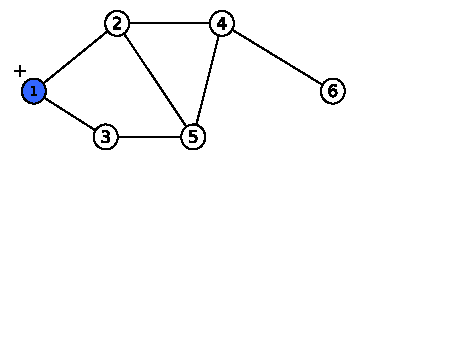
\includegraphics[width=\textwidth]{images/nodecharge1.png}
			\caption{}
			\label{particle1}
		\end{subfigure}~
		\begin{subfigure}[b]{0.3\textwidth}
			\includegraphics[width=\textwidth]{images/nodecharge11.png}
			\caption{}
			\label{polarity2}
		\end{subfigure}~ 
		\begin{subfigure}[b]{0.3\textwidth}
			\includegraphics[width=\textwidth]{images/nodecharge2.png}
			\caption{}
			\label{polarity3}
		\end{subfigure}
		\caption{ Illustration of how the polarisation analogy used as a motivation for the $k$-path Laplacian concept for networks. }
	\end{figure}
\end{itemize}
\end{frame}

\begin{frame}{Generalised Heat Diffusion Model Cont... }
\begin{itemize}
	\item $k$-path Laplacian Matrices are given by (Estrada et al., 2012)
	\begin{eqnarray}
	L_k(ij) = \begin{cases} -1 &\mbox{if } d_{i,j} = k, \\
	\delta_k(i) &\mbox{if } i = j,  \\
	0 & \text{otherwise},
	\end{cases}
	\end{eqnarray}\label{k-laplacian}
	where \\
	$d_{i,j}$ is the shortest path distance between nodes $i$ and $j$, \\
	$\delta_{k}(i)$ known as the $k$-path degree.
\end{itemize}
\end{frame}
\begin{frame}{$k$-path Laplacian Example}
	\begin{figure}[H]
		\centering
		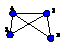
\includegraphics[width=0.25\textwidth]{images/compute-spanning.pdf}
		\captionof{figure}{ A network of size 4.}
		\label{spanning}
	\end{figure}
	
	\begin{eqnarray*}
		\mathbf{L_1(G)} = \begin{pmatrix}
			2 & -1 & 0 & -1 \\
			-1 & 3 & -1 & -1 \\
			0 & -1 & 2 & -1  \\
			-1 & -1 & -1 & 3
		\end{pmatrix}, \quad
		\mathbf{L_2(G)} = \begin{pmatrix}
			1 & 0 & -1 & 0 \\
			0 & 0 & 0 & 0 \\
			-1 & 0 & 1 & 0 \\
			0 & 0 & 0 & 0
		\end{pmatrix}
	\end{eqnarray*}
\end{frame}

\begin{frame}{Generalised Laplacian Matrix}
	\begin{itemize}
	\item The generalised Laplacian matrix, $L_G$, is given by
	\begin{equation}
	L_{G} = \sum_{k=1}^{\Delta} c_{k}L_{k}
	\end{equation}
	where $1 \leq \Delta \leq d_{max}$ and $c_k$ are the coefficients.
	
	\item  The values of $c_k$ are expected to give more weight to shorter than to the longer range interactions. Some commonly used co-efficients are $k^{-s}$, $e^{-\lambda k}$, etc.
	\end{itemize}
\end{frame}

\begin{frame}{Generalised Diffusion Model...cont...}
	\begin{figure}[!h]
		\centering
		\begin{subfigure}[b]{0.3\textwidth}
			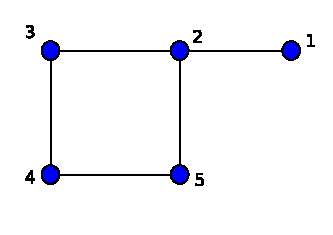
\includegraphics[width=\textwidth]{images/kenel-toymodel.pdf}
			\caption{}
			\label{toymodel}
		\end{subfigure}~
		\begin{subfigure}[b]{0.3\textwidth}
			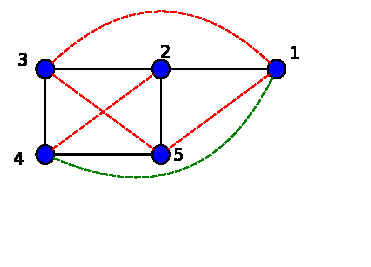
\includegraphics[width= \textwidth]{images/graph-longrange-demo.pdf}
			\caption{}
			\label{graph-longrange}
		\end{subfigure}
		\caption{(\subref{toymodel}) is a simple graph. (\subref{graph-longrange}) illustrates the long-range interaction on the graph.   }
		\label{}
	\end{figure}
\begin{itemize}
	\item The diffusion with longrange interactions is described by
	\begin{equation}
	\frac{d\boldsymbol{\phi}}{dt} =  -C\mathbf{L_G}\boldsymbol{\phi},  \quad \boldsymbol{\phi}(0) = \boldsymbol{\phi}_0 
	\end{equation}
\end{itemize}
\end{frame}

\section{Heat Kernel of a Graph}
\begin{frame}{Heat Kernel, $H_t$}
	\begin{block}{}
		\begin{itemize}
			\item The heat kernel is the fundamental solution of equation of the diffusion equation (\ref{heatequation}). 
%			\begin{equation}
%			\boldsymbol{\phi}(t) = e^{-c t \mathbf{L}} ~ \boldsymbol{\phi}_0
%			\end{equation} 
			\vspace{0.5cm}
			\pause
            \item It is obtained by exponentiating the Laplacian eigensystem and it is given by
			\begin{equation}
			H_t = e^{-c t \mathbf{L}} 
			\end{equation} 
			\vspace{0.5cm}
			\pause
			\item It literally describes the flow of substance (heat) across edges (direct interactions) in the graph.
		\end{itemize}
	\end{block}
\end{frame}
\begin{frame}{Trace of the Heat kernel}
	The trace of the heat kernel $Tr(H_t)$ is given by
		\begin{equation}
	Z(t) = Tr(H_t) = Tr(e^{(-\Lambda t)}) = \sum_{i=1}^{|V|} e^{-\lambda_i t},
	\label{kerneltrace}
	\end{equation}
	where $\lambda_i$ is the eigenvalue of the normalised Laplacian matrix.
	
	\begin{figure}[H]
		\centering
		\begin{subfigure}[b]{0.45\textwidth}
			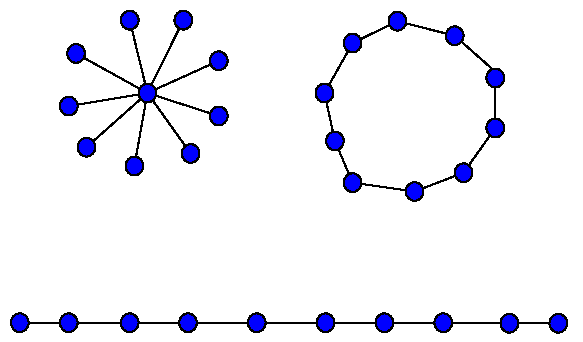
\includegraphics[width= \textwidth]{images/kernel-graphs.pdf}
			\caption{}
			\label{kernelgraphs}
		\end{subfigure}~
		\begin{subfigure}[b]{0.45\textwidth}
			\includegraphics[width= \textwidth]{images/Trace-kernel-plot}
			\caption{}
			\label{plot-kernel}
		\end{subfigure}
	\end{figure}
\end{frame}

\begin{frame}{Zeta Function}
	\begin{block}{}
	\begin{itemize}
	\item The Zeta function associated with the Laplacian eigenvalues is obtained by exponentiating and summing the reciprocal of the non-zero Laplacian eigenvalues. 
	\pause
	\vspace{0.5cm}
	\item It is thus defined by \cite{xiao2007kernel}
	\begin{equation}
	\zeta(s) = \sum_{\lambda_i \neq 0} \lambda_i ^{-s}.
	\end{equation} 
   \end{itemize}
\end{block}
\end{frame}



\begin{frame}{Application of Heat Kernel Invariants in Image Clustering}
	\begin{figure}[H]
		\centering
			\includegraphics[width= \textwidth]{images/GraphClustering.png}
			\caption{Illustration of Image Clustering process]}
	\end{figure}
	
\end{frame}

%\begin{frame}{Possible Extension of Laplacian Centrality}
%	\begin{itemize}
%		\item How the story will be with directed networks?
%		\begin{columns}
%			\begin{column}{0.5\textwidth}
%				\begin{center}
%					\begin{figure}
%						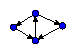
\includegraphics[width=0.85\textwidth]{images/directed-graph.pdf}
%						%\caption{Simple Directed graph }
%					\end{figure}
%				\end{center}
%			\end{column}
%			\begin{column}{0.45\textwidth}  
%				\begin{eqnarray*}
%					L &=& D_{out} - A \\
%					L &=& \begin{pmatrix}
%						2 & -1& 0& -1 \\
%						0 & 1& -1 & 0 \\
%						-1 & 0& 1 & 0 \\
%						0 & 0& -1 & 1 \\
%					\end{pmatrix}
%				\end{eqnarray*}
%			\end{column}
%		\end{columns}
%		\item To begin with, the Laplacian matrix of the directed network is not symmetric. This perhaps brings in a twist in the whole story.
%	\end{itemize}
%	
%\end{frame}


\begin{frame}{Summary}
	\begin{itemize}
		\item Introduction to Networks and network theory approach to Complex systems study.
		\item Laplacian matrix and its application namely Centrality measure and Diffusion.
		\item Heat kernel and its use in graph characterisation
		\item Image clustering using heat kernel invariants
		\item Further work: Considering other heat kernel invariants with aim of obtaining better image clustering.
	\end{itemize}
	
\end{frame}


\begin{frame}[allowframebreaks]
	\frametitle<presentation>{References}  
	\begin{thebibliography}{99} 
		
		\bibitem{newman2010} Newman, M., 2010. Networks: an introduction. Oxford university press.
		
		\bibitem{estrada2011epidemic} Estrada, E., Kalala-Mutombo, F. and Valverde-Colmeiro, A., 2011. Epidemic spreading in networks with nonrandom long-range interactions. Physical Review E, 84(3), p.036110.
		
		\bibitem{estrada2012path} Estrada, E., 2012. Path Laplacian matrices: introduction and application to the analysis of consensus in networks. Linear Algebra and its Applications, 436(9), pp.3373-3391.
		
		\bibitem{estrada2017long} Estrada, E., Hameed, E., Hatano, N. and Langer, M., 2017. Path Laplacian operators and superdiffusive processes on graphs. I. One-dimensional case. Linear Algebra and its Applications, 523, pp.307-334.
		
		\bibitem{xiao2007kernel}Bai, X., 2007. Heat Kernal Analysis on Graphs. University of York, Department of Computer Science.
		
		\bibitem{xiao2009graph} Xiao, B., Hancock, E.R. and Wilson, R.C., 2009. Graph characteristics from the heat kernel trace. Pattern Recognition, 42(11), pp.2589-2606.
		
%		
%		\bibitem{wiki} \begin{verbatim} http://en.wikibooks.org/wiki/LaTeX \end{verbatim}
		
	\end{thebibliography}
	
\end{frame}

\begin{frame}{Acknowledgements}
	\begin{itemize}
		\item AIMS, South Africa \& Stellenbosch University
		\item AIMS, Senegal
	\end{itemize}
	
\end{frame}
%------------------------------------------------

%\begin{frame}
%\frametitle{References}
%\footnotesize{
%\begin{thebibliography}{99} % Beamer does not support BibTeX so references must be inserted manually as below
%\bibitem[Smith, 2012]{p1} John Smith (2012)
%\newblock Title of the publication
%\newblock \emph{Journal Name} 12(3), 45 -- 678.
%\end{thebibliography}
%}
%\end{frame}

%\begin{frame}
%	\movie[height = 0.6\textwidth, width = 0.8\textwidth, poster, showcontrols]{}{movie.mp4} 
%\end{frame}

%\begin{frame}[allowframebreaks]
%	\frametitle{References}
%	
%	\nocite{*}
%	\bibliographystyle{abbrv}
%	\bibliography{bmsreferences}
%\end{frame}

%------------------------------------------------

\begin{frame}[noframenumbering, plain]
\begin{figure}[!h]
	\centering	
		\includegraphics[width=\textwidth]{images/merci.jpg}
	\end{figure}
\end{frame}

%----------------------------------------------------------------------------------------

\end{document} 